\documentclass[class=jsarticle, crop=false, dvipdfmx, fleqn]{standalone}
\input{/Users/User/Documents/University/report_template/preamble/preamble}
\begin{document}

\section*{宿題1}

2つのクラス\(c_1,\ c_2\)からそれぞれ得た標本\(x_1,\ x_2\)について,
条件付確率密度\(p(x|c_i\))を,
パルゼンウィンドウ法(カーネル関数として正規分布と超立方体両方)と
k近傍法(様々な\(k\)について)で求め,図示する。
また,その事後確率\(p(c_i|x)\)も図示する。

図\ref{fig:x1},\ref{fig:x2}にそれぞれ\(x_1,\ x_2\)のヒストグラムを示す。

\begin{figure}
    \centering
    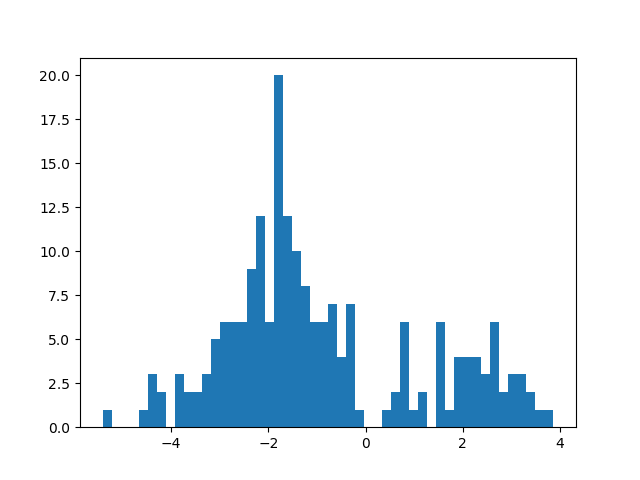
\includegraphics[clip, width=8cm]{../figures/x1}
    \caption{\(x_1\)のヒストグラム}
    \label{fig:x1}
\end{figure}

\begin{figure}
    \centering
    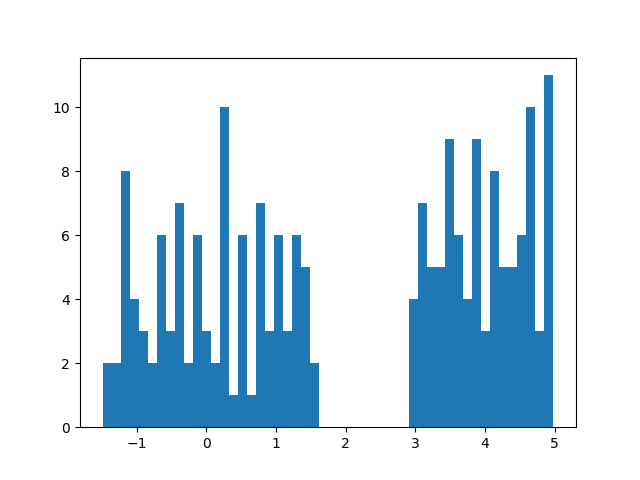
\includegraphics[clip, width=8cm]{../figures/x2}
    \caption{\(x_2\)のヒストグラム}
    \label{fig:x2}
\end{figure}



\subsection*{プログラム}

プログラムの本体は\pageref{listing:assignment1}ページのListing \ref{listing:assignment1}に示した。
以下に簡単なプログラムの説明を示す。

\begin{itemize}
    \item load \\
        .matファイルからデータを読み出し,
        \(x_1,\ x_2\)のデータを返す。
    \item plot\_data \\
        \(x_1,\ x_2\)それぞれのヒストグラムをプロットする。
    \item normal\_distribution \\
        正規分布の確率密度を返す。
        parzen法におけるカーネル関数として用いる。
    \item hypercube \\
        超立方体の確率密度を返す。
        parzen法におけるカーネル関数として用いる。
    \item conditional\_probability\_parzen \\
        parzen法における条件付確率を求める。
    \item conditiona\_probability\_kmeans \\
        k近傍法における条件付確率を求める。
        距離関数には絶対値を用いる。
    \item \_nonparametric\_method \\
        parzen法とk近傍法で\(x_1,\ x_2\)の条件付確率と事後確率を求めてプロットするときの,
        共通する部分をまとめた関数。
    \item parzen \\
        parzen法で\(x_1,\ x_2\)の条件付確率と事後確率を求めてプロットする。
    \item kmeans \\
        k近傍法で\(x_1,\ x_2\)の条件付確率と事後確率を求めてプロットする。
    \item main \\
        上記の関数をまとめて実行する関数。
\end{itemize}



\subsection*{結果}

parzen法にて正規分布をカーネル関数として用いたときの結果を図\ref{fig:parzen_norm_result}に,
超立方体をカーネル関数として用いたときの結果を図\ref{fig:parzen_hypercube_result}に,
k近傍法の結果を図\ref{fig:kmeans_result}に示す。
バンド幅\(h\)とクラスタに含まれるサンプル数\(k\)は,
図に示した値について実験した。

\begin{figure}
    \centering
    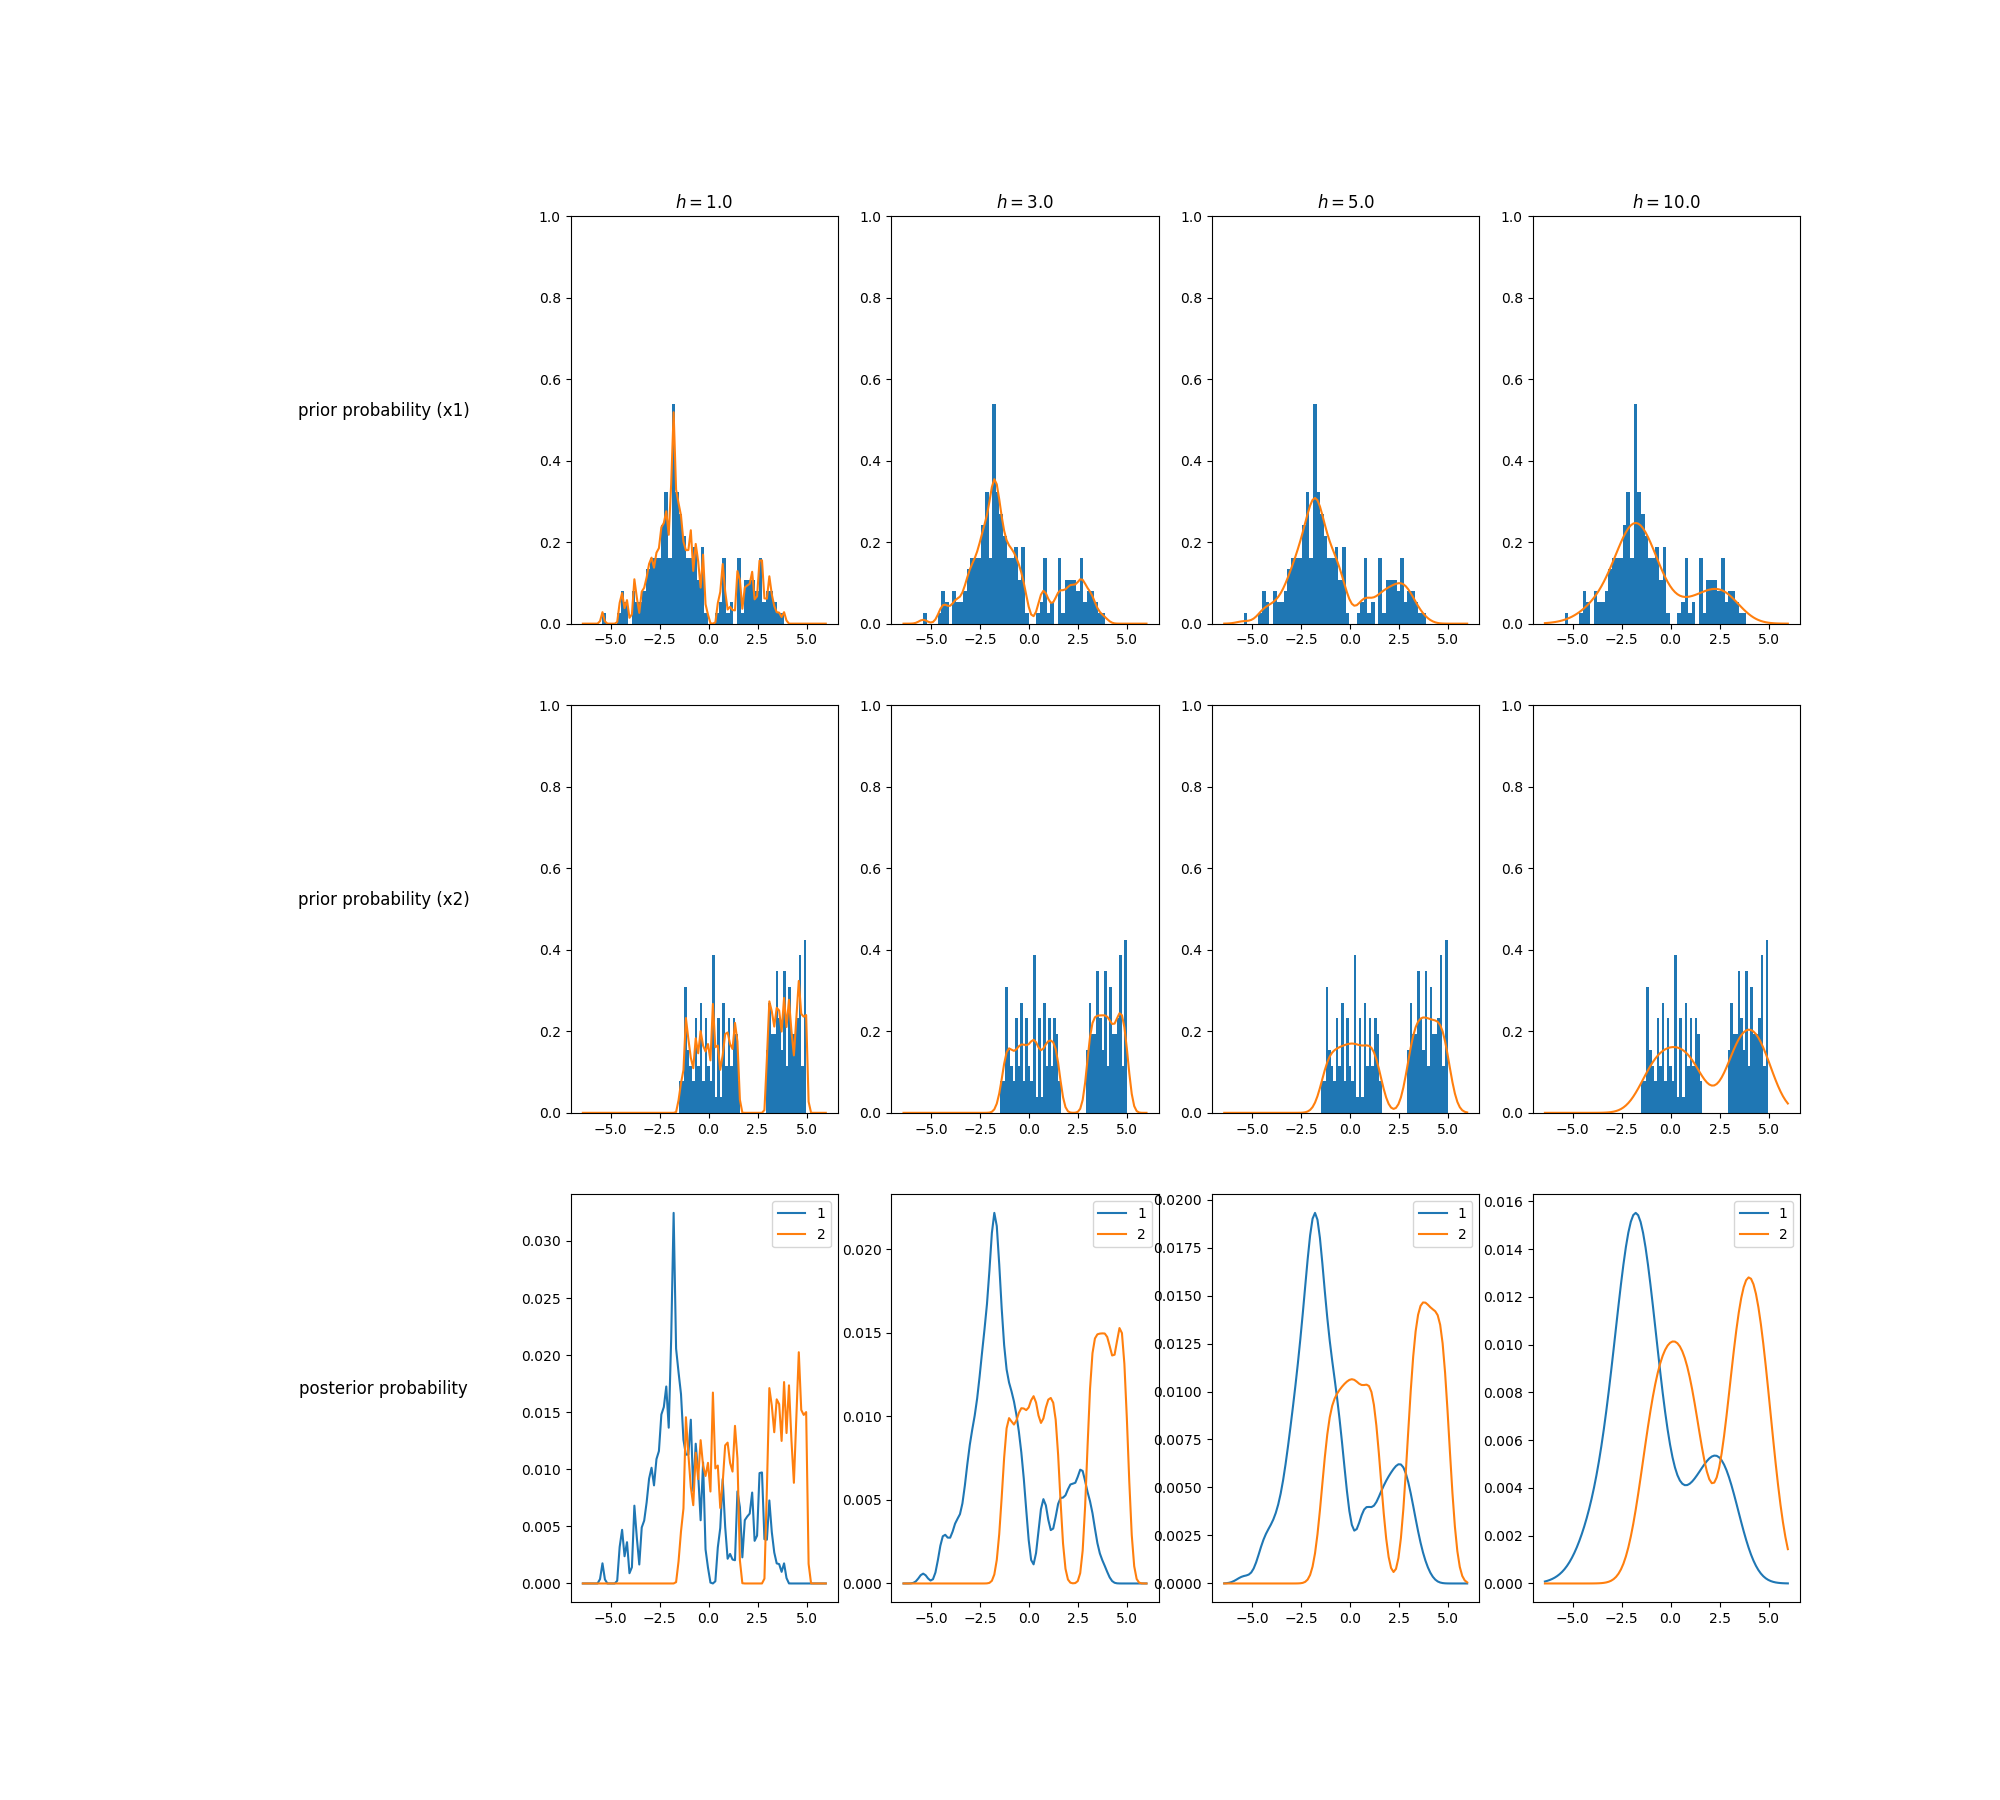
\includegraphics[clip, width=18cm, trim=200 72 0 0]{../figures/parzen_norm_result}
    \caption{parzen法にて正規分布をカーネル関数として用いたときの結果}
    \label{fig:parzen_norm_result}
\end{figure}

\begin{figure}
    \centering
    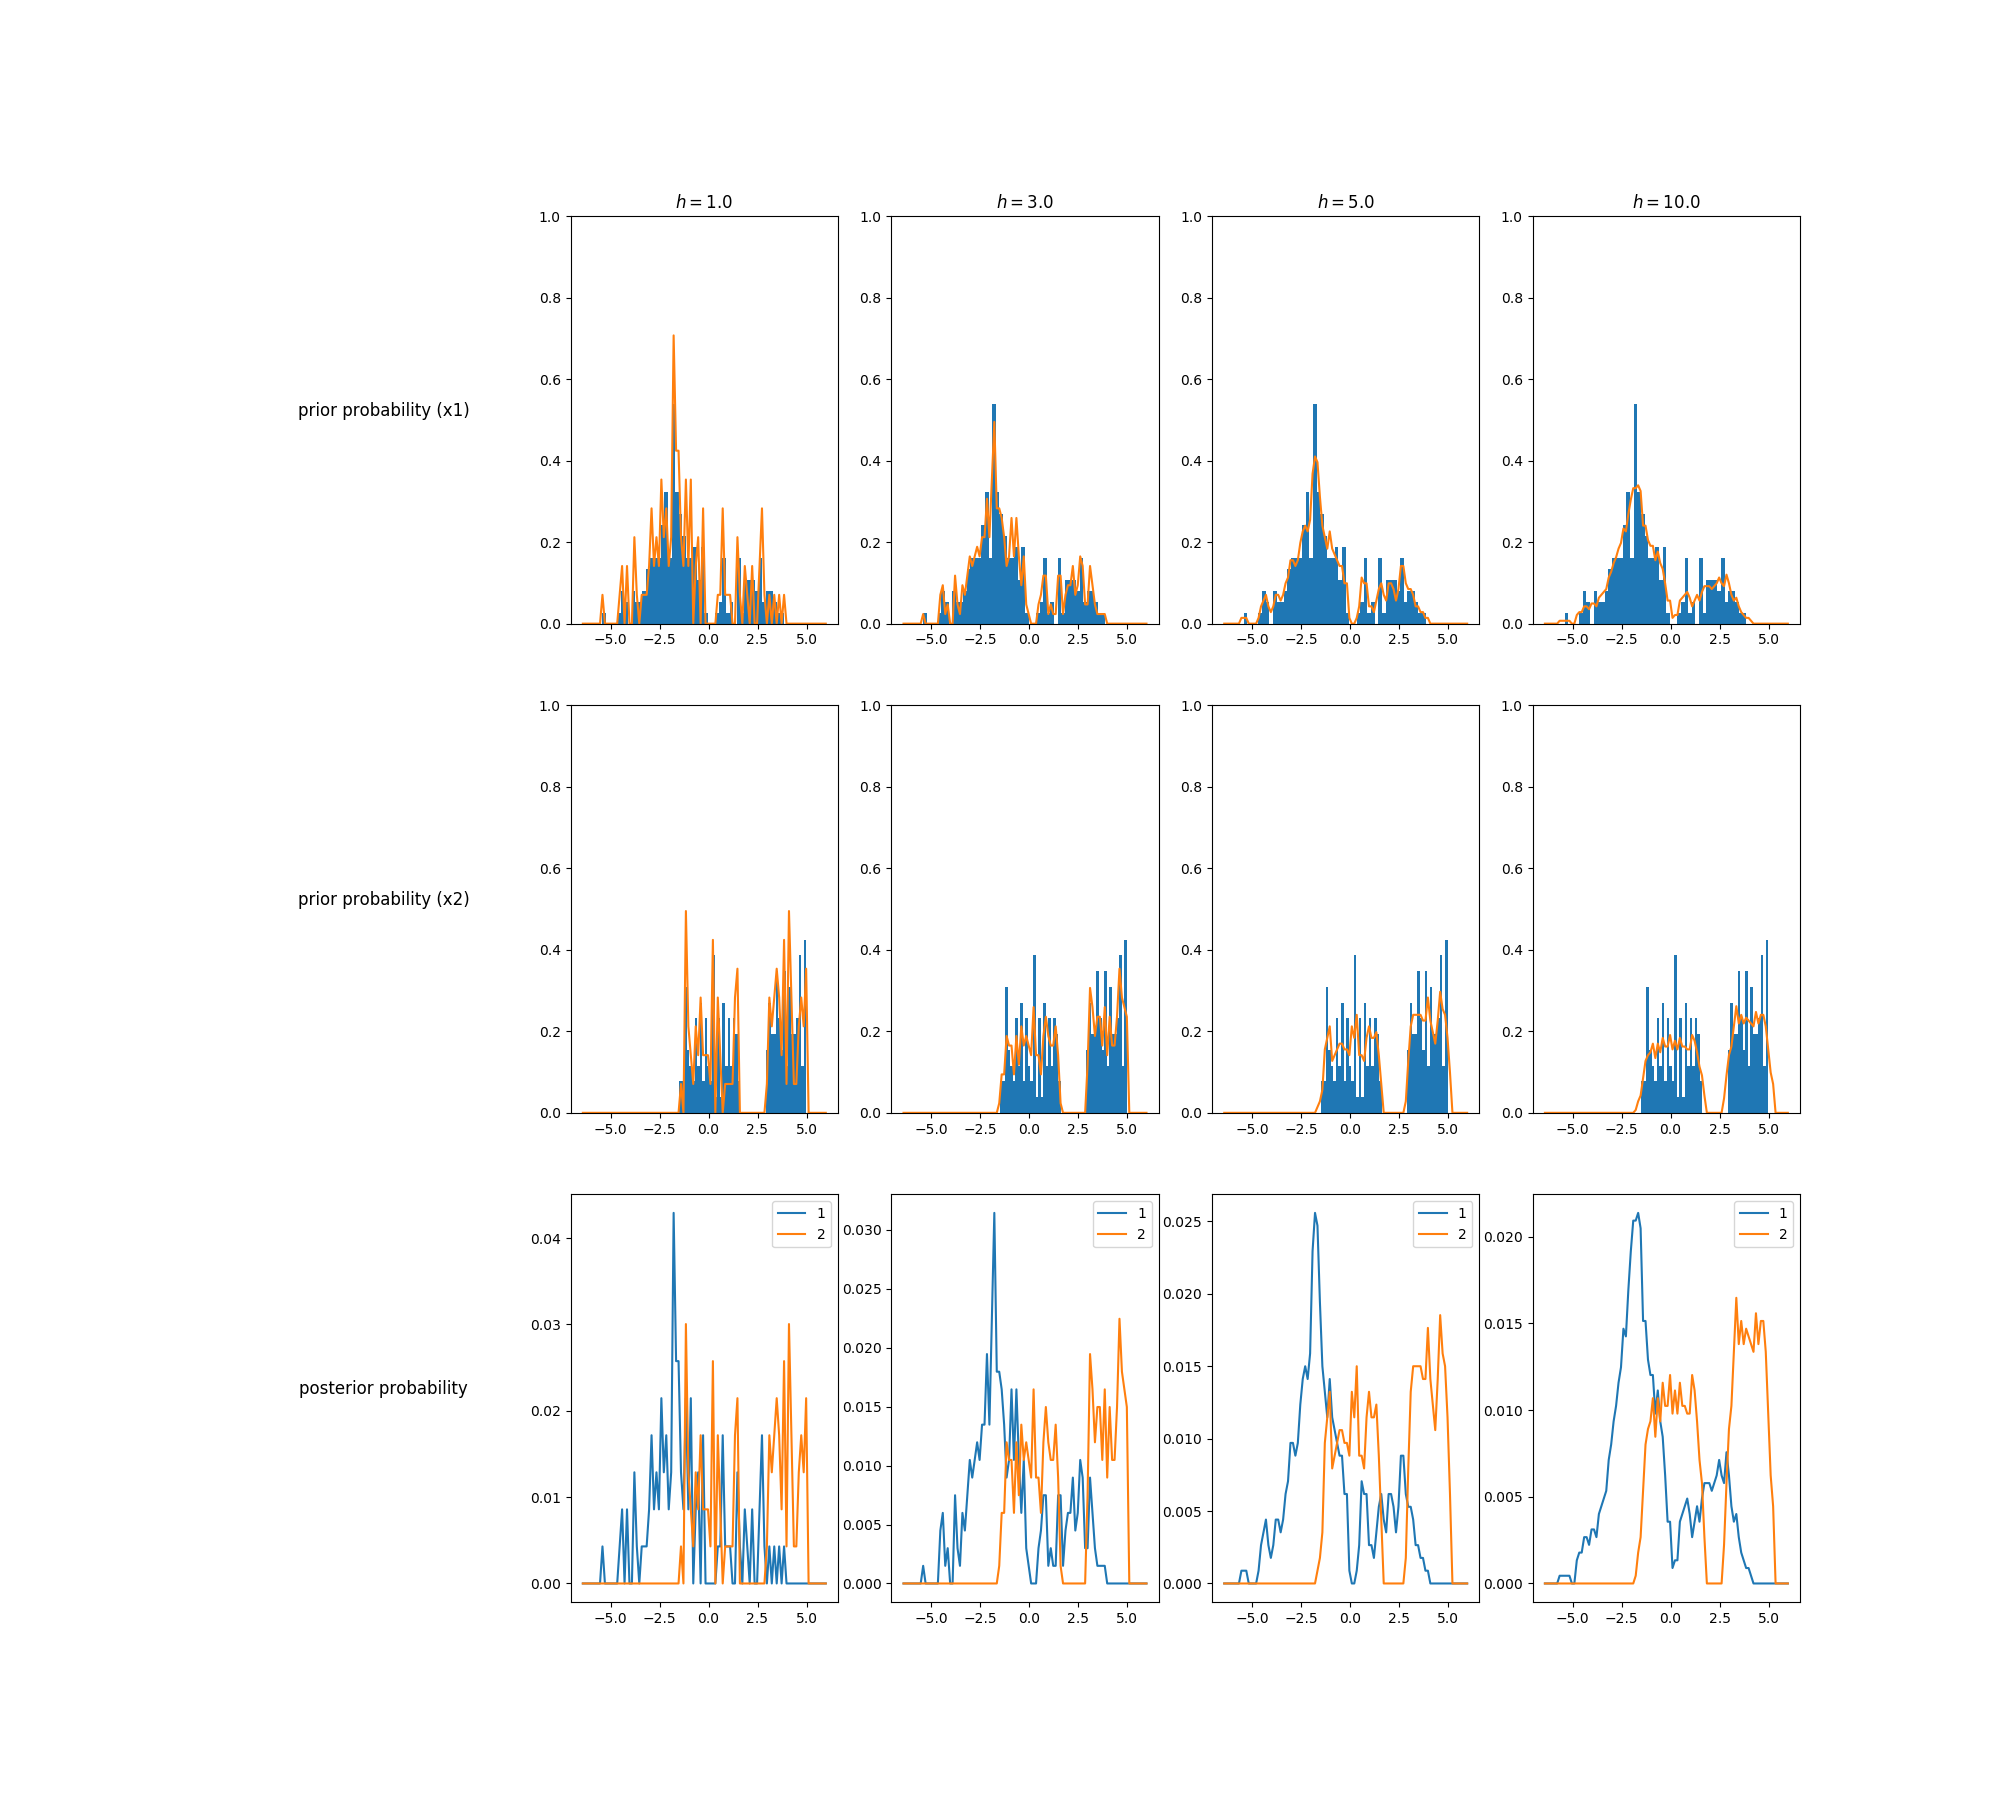
\includegraphics[clip, width=18cm, trim=200 72 0 0]{../figures/parzen_hypercube_result}
    \caption{parzen法にて超立方体をカーネル関数として用いたときの結果}
    \label{fig:parzen_hypercube_result}
\end{figure}

\begin{figure}
    \centering
    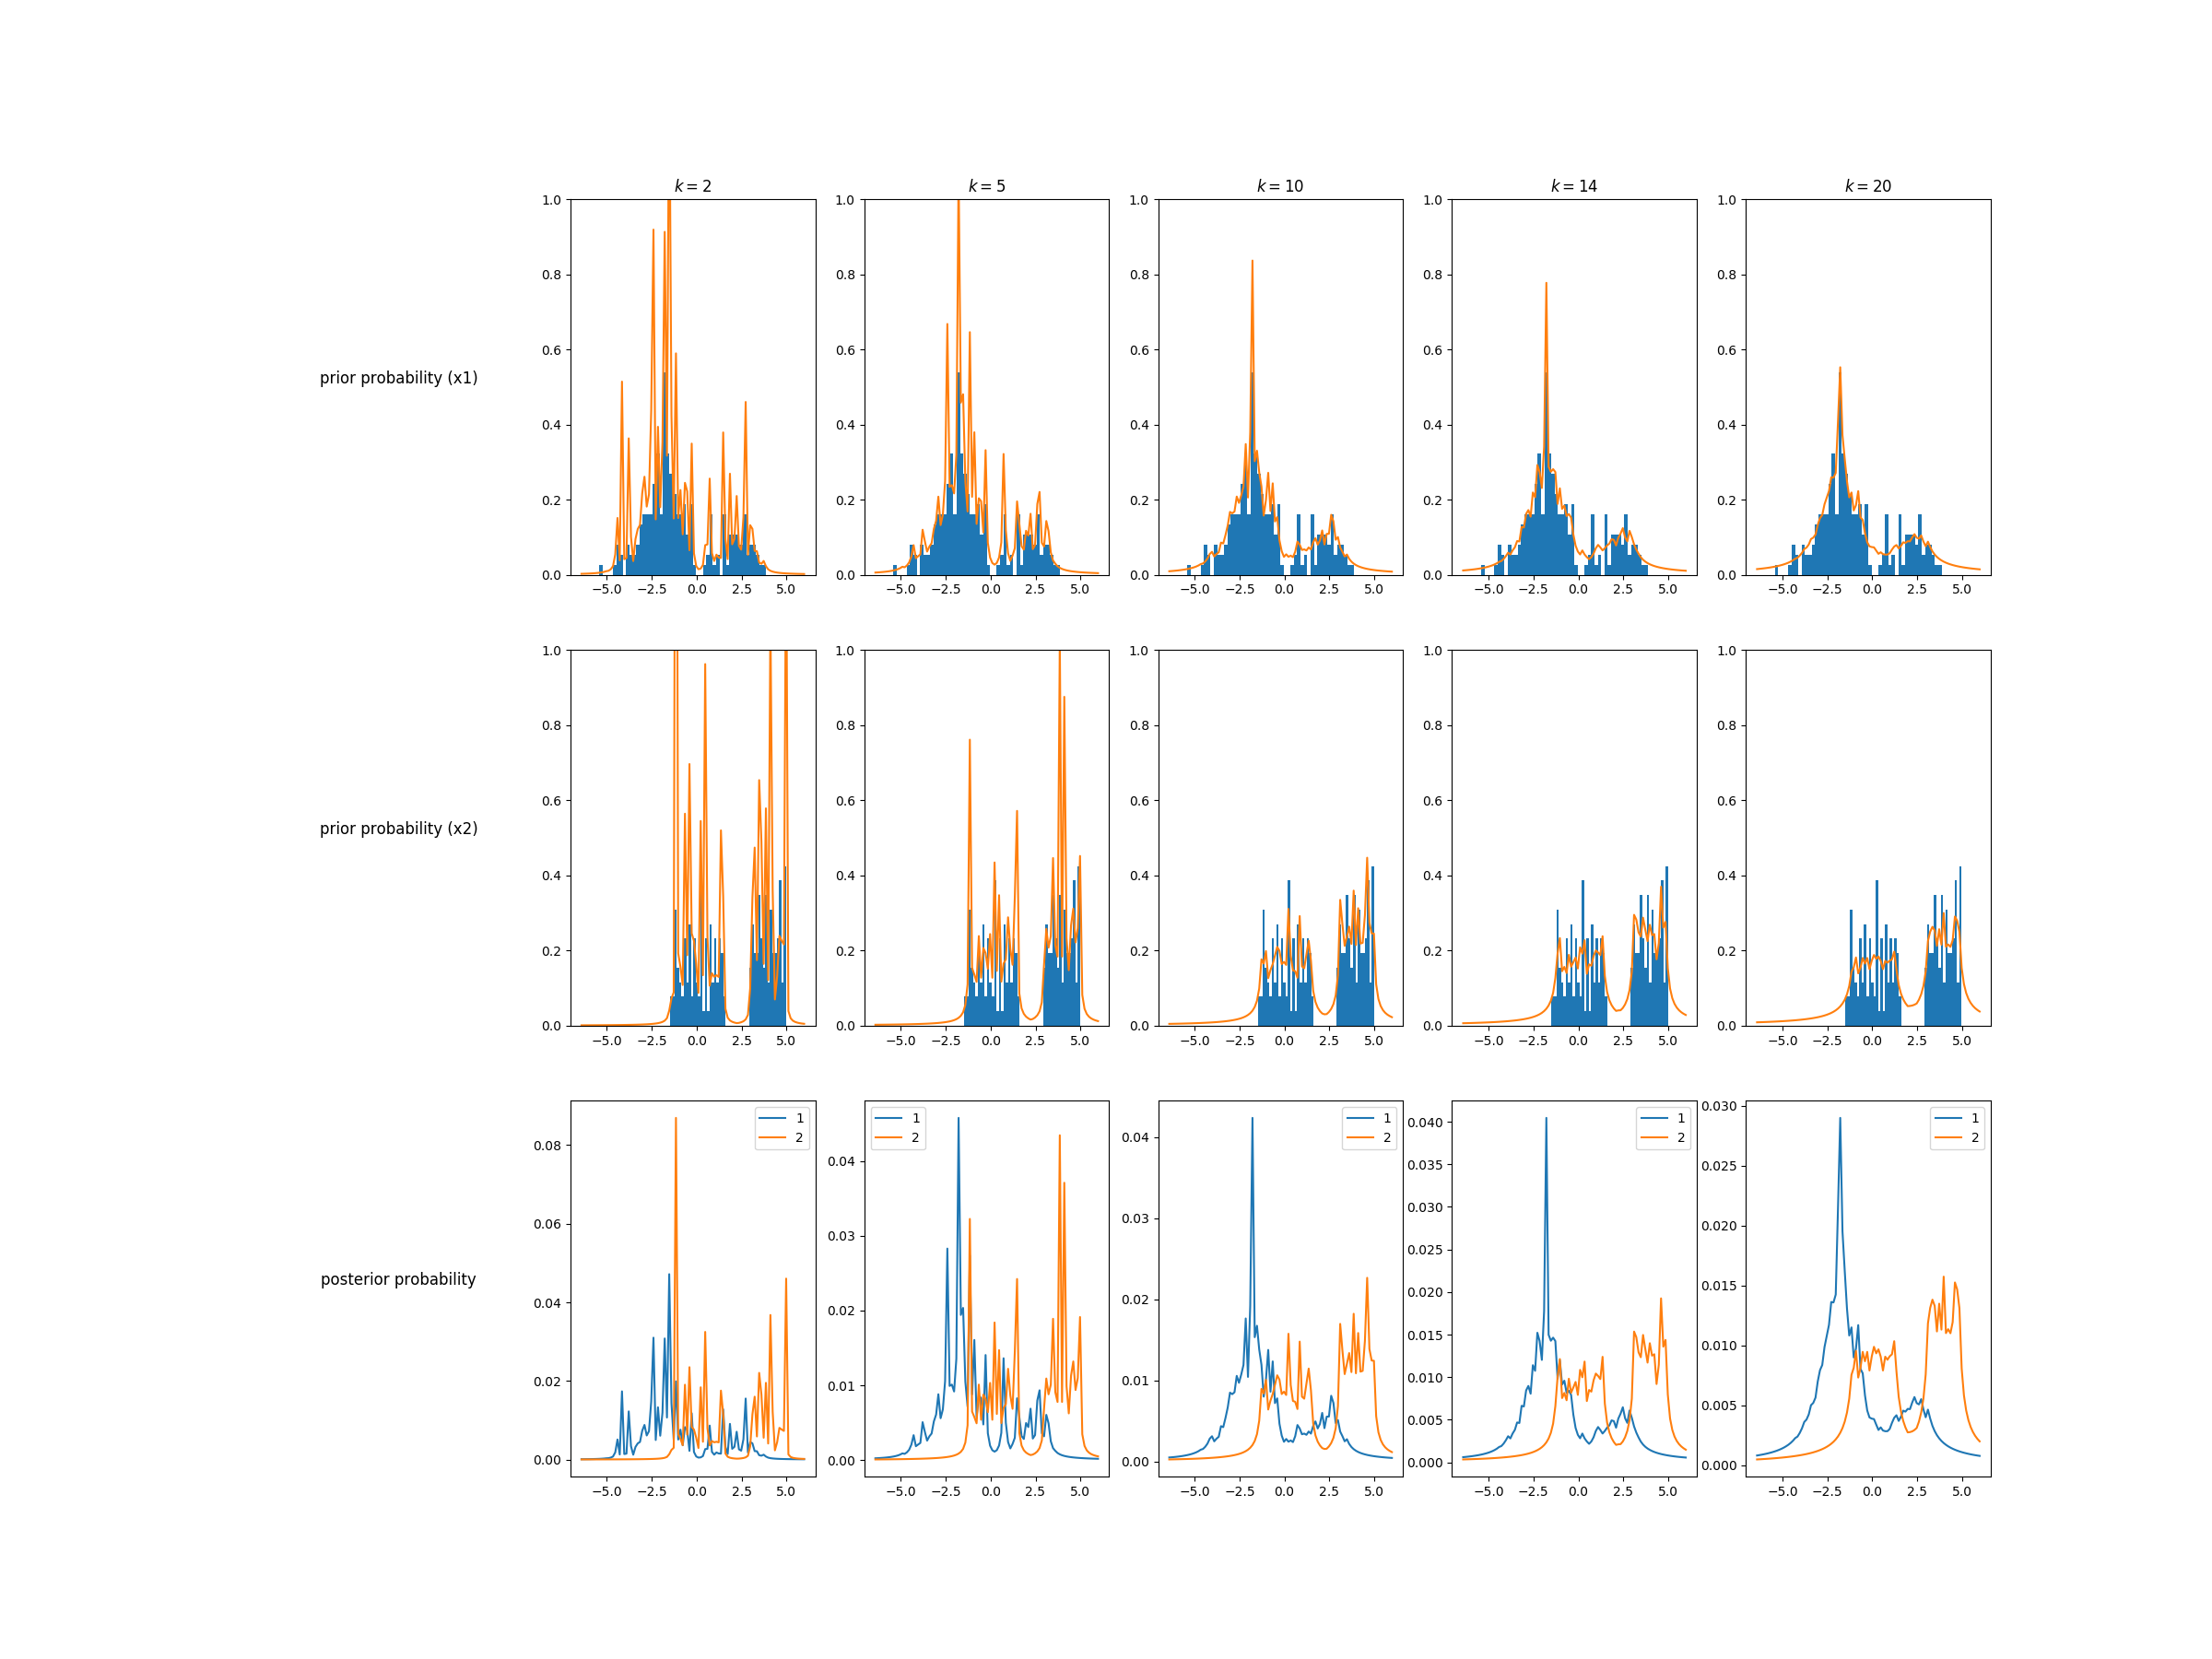
\includegraphics[clip, width=18cm, trim=200 72 0 0]{../figures/kmeans_result}
    \caption{k近傍法の結果}
    \label{fig:kmeans_result}
\end{figure}



\subsection*{考察}

parzen法において正規分布をカーネル関数として用いた場合は,
バンド幅\(h = 3\)でもかなり滑らかな確率密度関数が得られていたが,
超立方体を用いた場合は\(h = 10\)でもあまり滑らかにはならなかった。
これは,
正規分布の領域は分散の影響で\(x\)に対し滑らかにしか変化しないのに対し,
超立方体はその領域の内と外をきっぱりと分けてしまう,
つまり\(x\)に対し不連続に変化するため,
当然ともいえる。
実際,\(x_2\)のような,不連続(に見えるよう)な分布について,バンド幅3のものを見れば,
正規分布ではデータが存在しない部分でも確率密度関数の値が大きくなってしまっているが,
超立方体ではそのような部分はほとんど見られない。
逆に,\(x_1\)のような,\(x\)に対し滑らかに変化しているような分布については,
正規分布はうまく真の分布を近似しているように見えるが,
超立方体ではノイズの影響が大きく出てしまっている。

k近傍法については,
\(k\)が小さいときは値が発散してしまっていて,
ある程度大きくすると(\(k \ge 10\)),
真の分布に近づけている。



\end{document}
